\documentclass[twoside]{book}

% Packages required by doxygen
\usepackage{fixltx2e}
\usepackage{calc}
\usepackage{doxygen}
\usepackage[export]{adjustbox} % also loads graphicx
\usepackage{graphicx}
\usepackage[utf8]{inputenc}
\usepackage{makeidx}
\usepackage{multicol}
\usepackage{multirow}
\PassOptionsToPackage{warn}{textcomp}
\usepackage{textcomp}
\usepackage[nointegrals]{wasysym}
\usepackage[table]{xcolor}

% Font selection
\usepackage[T1]{fontenc}
\usepackage[scaled=.90]{helvet}
\usepackage{courier}
\usepackage{amssymb}
\usepackage{sectsty}
\renewcommand{\familydefault}{\sfdefault}
\allsectionsfont{%
  \fontseries{bc}\selectfont%
  \color{darkgray}%
}
\renewcommand{\DoxyLabelFont}{%
  \fontseries{bc}\selectfont%
  \color{darkgray}%
}
\newcommand{\+}{\discretionary{\mbox{\scriptsize$\hookleftarrow$}}{}{}}

% Page & text layout
\usepackage{geometry}
\geometry{%
  a4paper,%
  top=2.5cm,%
  bottom=2.5cm,%
  left=2.5cm,%
  right=2.5cm%
}
\tolerance=750
\hfuzz=15pt
\hbadness=750
\setlength{\emergencystretch}{15pt}
\setlength{\parindent}{0cm}
\setlength{\parskip}{3ex plus 2ex minus 2ex}
\makeatletter
\renewcommand{\paragraph}{%
  \@startsection{paragraph}{4}{0ex}{-1.0ex}{1.0ex}{%
    \normalfont\normalsize\bfseries\SS@parafont%
  }%
}
\renewcommand{\subparagraph}{%
  \@startsection{subparagraph}{5}{0ex}{-1.0ex}{1.0ex}{%
    \normalfont\normalsize\bfseries\SS@subparafont%
  }%
}
\makeatother

% Headers & footers
\usepackage{fancyhdr}
\pagestyle{fancyplain}
\fancyhead[LE]{\fancyplain{}{\bfseries\thepage}}
\fancyhead[CE]{\fancyplain{}{}}
\fancyhead[RE]{\fancyplain{}{\bfseries\leftmark}}
\fancyhead[LO]{\fancyplain{}{\bfseries\rightmark}}
\fancyhead[CO]{\fancyplain{}{}}
\fancyhead[RO]{\fancyplain{}{\bfseries\thepage}}
\fancyfoot[LE]{\fancyplain{}{}}
\fancyfoot[CE]{\fancyplain{}{}}
\fancyfoot[RE]{\fancyplain{}{\bfseries\scriptsize Generated by Doxygen }}
\fancyfoot[LO]{\fancyplain{}{\bfseries\scriptsize Generated by Doxygen }}
\fancyfoot[CO]{\fancyplain{}{}}
\fancyfoot[RO]{\fancyplain{}{}}
\renewcommand{\footrulewidth}{0.4pt}
\renewcommand{\chaptermark}[1]{%
  \markboth{#1}{}%
}
\renewcommand{\sectionmark}[1]{%
  \markright{\thesection\ #1}%
}

% Indices & bibliography
\usepackage{natbib}
\usepackage[titles]{tocloft}
\setcounter{tocdepth}{3}
\setcounter{secnumdepth}{5}
\makeindex

% Hyperlinks (required, but should be loaded last)
\usepackage{ifpdf}
\ifpdf
  \usepackage[pdftex,pagebackref=true]{hyperref}
\else
  \usepackage[ps2pdf,pagebackref=true]{hyperref}
\fi
\hypersetup{%
  colorlinks=true,%
  linkcolor=blue,%
  citecolor=blue,%
  unicode%
}

% Custom commands
\newcommand{\clearemptydoublepage}{%
  \newpage{\pagestyle{empty}\cleardoublepage}%
}

\usepackage{caption}
\captionsetup{labelsep=space,justification=centering,font={bf},singlelinecheck=off,skip=4pt,position=top}

%===== C O N T E N T S =====

\begin{document}

% Titlepage & ToC
\hypersetup{pageanchor=false,
             bookmarksnumbered=true,
             pdfencoding=unicode
            }
\pagenumbering{roman}
\begin{titlepage}
\vspace*{7cm}
\begin{center}%
{\Large Space Intruders \\[1ex]\large 0.\+1 }\\
\vspace*{1cm}
{\large Generated by Doxygen 1.8.11}\\
\end{center}
\end{titlepage}
\clearemptydoublepage
\tableofcontents
\clearemptydoublepage
\pagenumbering{arabic}
\hypersetup{pageanchor=true}

%--- Begin generated contents ---
\chapter{Hierarchical Index}
\section{Class Hierarchy}
This inheritance list is sorted roughly, but not completely, alphabetically\+:\begin{DoxyCompactList}
\item \contentsline{section}{Input\+Listener}{\pageref{class_input_listener}}{}
\begin{DoxyCompactList}
\item \contentsline{section}{Niveau}{\pageref{class_niveau}}{}
\end{DoxyCompactList}
\item \contentsline{section}{Screen}{\pageref{class_screen}}{}
\begin{DoxyCompactList}
\item \contentsline{section}{Niveau}{\pageref{class_niveau}}{}
\end{DoxyCompactList}
\item \contentsline{section}{Space\+Intruders}{\pageref{class_space_intruders}}{}
\end{DoxyCompactList}

\chapter{Class Index}
\section{Class List}
Here are the classes, structs, unions and interfaces with brief descriptions\+:\begin{DoxyCompactList}
\item\contentsline{section}{\hyperlink{class_input_listener}{Input\+Listener} \\*Classe gérant les entrées }{\pageref{class_input_listener}}{}
\item\contentsline{section}{\hyperlink{class_niveau}{Niveau} \\*Classe représentant un niveau de jeu }{\pageref{class_niveau}}{}
\item\contentsline{section}{\hyperlink{class_screen}{Screen} \\*Classe representant un écran de jeu }{\pageref{class_screen}}{}
\item\contentsline{section}{\hyperlink{class_space_intruders}{Space\+Intruders} \\*Classe representant le jeu }{\pageref{class_space_intruders}}{}
\end{DoxyCompactList}

\chapter{File Index}
\section{File List}
Here is a list of all files with brief descriptions\+:\begin{DoxyCompactList}
\item\contentsline{section}{\hyperlink{_input_listener_8hpp}{Input\+Listener.\+hpp} \\*Classe gérant les entrées }{\pageref{_input_listener_8hpp}}{}
\item\contentsline{section}{\hyperlink{main_8cpp}{main.\+cpp} }{\pageref{main_8cpp}}{}
\item\contentsline{section}{\hyperlink{_niveau_8cpp}{Niveau.\+cpp} }{\pageref{_niveau_8cpp}}{}
\item\contentsline{section}{\hyperlink{_niveau_8hpp}{Niveau.\+hpp} \\*Classe représentant un niveau de jeu }{\pageref{_niveau_8hpp}}{}
\item\contentsline{section}{\hyperlink{_screen_8hpp}{Screen.\+hpp} \\*Classe représenatnt un écran de jeu }{\pageref{_screen_8hpp}}{}
\item\contentsline{section}{\hyperlink{_space_intruders_8cpp}{Space\+Intruders.\+cpp} }{\pageref{_space_intruders_8cpp}}{}
\item\contentsline{section}{\hyperlink{_space_intruders_8hpp}{Space\+Intruders.\+hpp} \\*Classe principale du jeu }{\pageref{_space_intruders_8hpp}}{}
\end{DoxyCompactList}

\chapter{Class Documentation}
\hypertarget{class_input_listener}{}\section{Input\+Listener Interface Reference}
\label{class_input_listener}\index{Input\+Listener@{Input\+Listener}}


Classe gérant les entrées.  




{\ttfamily \#include $<$Input\+Listener.\+hpp$>$}



Inheritance diagram for Input\+Listener\+:\nopagebreak
\begin{figure}[H]
\begin{center}
\leavevmode
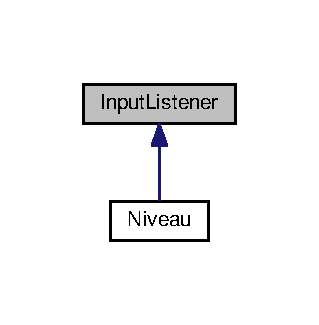
\includegraphics[width=153pt]{class_input_listener__inherit__graph}
\end{center}
\end{figure}
\subsection*{Public Member Functions}
\begin{DoxyCompactItemize}
\item 
virtual void \hyperlink{class_input_listener_a415245dec47d3e80be64b779859a90c9}{keys\+Down} (std\+::map$<$ double, bool $>$ \&k)=0
\begin{DoxyCompactList}\small\item\em Méthodes transmettant les infos sur les clés clavier juste pressées. \end{DoxyCompactList}\item 
virtual void \hyperlink{class_input_listener_a0a9bea1bfdcb82a827a48ad35d692600}{keys\+Hold} (std\+::map$<$ double, bool $>$ \&k)=0
\begin{DoxyCompactList}\small\item\em Méthode transmettant les infos sur les clés clavier actuellement pressées. \end{DoxyCompactList}\item 
virtual void \hyperlink{class_input_listener_a188edcf4460b5db1081ddd7b9f271175}{keys\+Up} (std\+::map$<$ double, bool $>$ \&k)=0
\begin{DoxyCompactList}\small\item\em Méthodes transmettant les infos sur les clés clavier juste relachées. \end{DoxyCompactList}\end{DoxyCompactItemize}


\subsection{Detailed Description}
Classe gérant les entrées. 

Definition at line 17 of file Input\+Listener.\+hpp.



\subsection{Member Function Documentation}
\index{Input\+Listener@{Input\+Listener}!keys\+Down@{keys\+Down}}
\index{keys\+Down@{keys\+Down}!Input\+Listener@{Input\+Listener}}
\subsubsection[{\texorpdfstring{keys\+Down(std\+::map$<$ double, bool $>$ \&k)=0}{keysDown(std::map< double, bool > &k)=0}}]{\setlength{\rightskip}{0pt plus 5cm}virtual void Input\+Listener\+::keys\+Down (
\begin{DoxyParamCaption}
\item[{std\+::map$<$ double, bool $>$ \&}]{k}
\end{DoxyParamCaption}
)\hspace{0.3cm}{\ttfamily [pure virtual]}}\hypertarget{class_input_listener_a415245dec47d3e80be64b779859a90c9}{}\label{class_input_listener_a415245dec47d3e80be64b779859a90c9}


Méthodes transmettant les infos sur les clés clavier juste pressées. 


\begin{DoxyParams}{Parameters}
{\em k} & \+: Clés juste pressées \\
\hline
\end{DoxyParams}


Implemented in \hyperlink{class_niveau_a05eaf847a4d649a133d9259c0b9b2e2b}{Niveau}.

\index{Input\+Listener@{Input\+Listener}!keys\+Hold@{keys\+Hold}}
\index{keys\+Hold@{keys\+Hold}!Input\+Listener@{Input\+Listener}}
\subsubsection[{\texorpdfstring{keys\+Hold(std\+::map$<$ double, bool $>$ \&k)=0}{keysHold(std::map< double, bool > &k)=0}}]{\setlength{\rightskip}{0pt plus 5cm}virtual void Input\+Listener\+::keys\+Hold (
\begin{DoxyParamCaption}
\item[{std\+::map$<$ double, bool $>$ \&}]{k}
\end{DoxyParamCaption}
)\hspace{0.3cm}{\ttfamily [pure virtual]}}\hypertarget{class_input_listener_a0a9bea1bfdcb82a827a48ad35d692600}{}\label{class_input_listener_a0a9bea1bfdcb82a827a48ad35d692600}


Méthode transmettant les infos sur les clés clavier actuellement pressées. 


\begin{DoxyParams}{Parameters}
{\em k} & \+: Clés actuellement pressées \\
\hline
\end{DoxyParams}


Implemented in \hyperlink{class_niveau_a3730fe148bcfc20c96121769a48a0024}{Niveau}.

\index{Input\+Listener@{Input\+Listener}!keys\+Up@{keys\+Up}}
\index{keys\+Up@{keys\+Up}!Input\+Listener@{Input\+Listener}}
\subsubsection[{\texorpdfstring{keys\+Up(std\+::map$<$ double, bool $>$ \&k)=0}{keysUp(std::map< double, bool > &k)=0}}]{\setlength{\rightskip}{0pt plus 5cm}virtual void Input\+Listener\+::keys\+Up (
\begin{DoxyParamCaption}
\item[{std\+::map$<$ double, bool $>$ \&}]{k}
\end{DoxyParamCaption}
)\hspace{0.3cm}{\ttfamily [pure virtual]}}\hypertarget{class_input_listener_a188edcf4460b5db1081ddd7b9f271175}{}\label{class_input_listener_a188edcf4460b5db1081ddd7b9f271175}


Méthodes transmettant les infos sur les clés clavier juste relachées. 


\begin{DoxyParams}{Parameters}
{\em k} & \+: Clés juste relachée \\
\hline
\end{DoxyParams}


Implemented in \hyperlink{class_niveau_aceab76f09227e16b5dcdbb5ae0534ce9}{Niveau}.



The documentation for this interface was generated from the following file\+:\begin{DoxyCompactItemize}
\item 
\hyperlink{_input_listener_8hpp}{Input\+Listener.\+hpp}\end{DoxyCompactItemize}

\hypertarget{class_niveau}{}\section{Niveau Class Reference}
\label{class_niveau}\index{Niveau@{Niveau}}


Classe représentant un niveau de jeu.  




{\ttfamily \#include $<$Niveau.\+hpp$>$}



Inheritance diagram for Niveau\+:\nopagebreak
\begin{figure}[H]
\begin{center}
\leavevmode
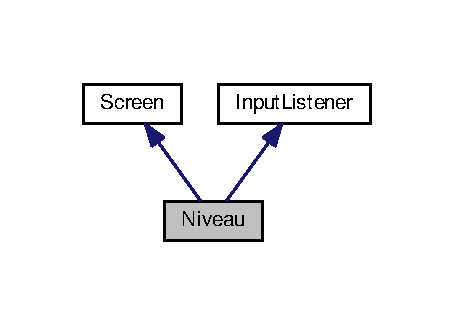
\includegraphics[width=218pt]{class_niveau__inherit__graph}
\end{center}
\end{figure}


Collaboration diagram for Niveau\+:\nopagebreak
\begin{figure}[H]
\begin{center}
\leavevmode
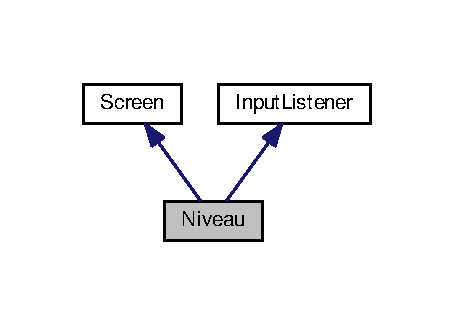
\includegraphics[width=218pt]{class_niveau__coll__graph}
\end{center}
\end{figure}
\subsection*{Public Member Functions}
\begin{DoxyCompactItemize}
\item 
\hyperlink{class_niveau_a0e9bc3e28ce24702949556c741a28bc5}{Niveau} (\hyperlink{class_space_intruders}{Space\+Intruders} $\ast$jeu)
\begin{DoxyCompactList}\small\item\em Construit un niveau. \end{DoxyCompactList}\item 
\hyperlink{class_niveau_ad5a39e5e034a061774564e145eb7cf61}{$\sim$\+Niveau} ()
\begin{DoxyCompactList}\small\item\em Detruit un niveau. \end{DoxyCompactList}\item 
void \hyperlink{class_niveau_a287b7fc08a2d7102008c134a72462d4f}{update} (float delta)
\begin{DoxyCompactList}\small\item\em Méthode appelée a chaque boucle de jeu. \end{DoxyCompactList}\item 
void \hyperlink{class_niveau_acde898f3c32db22484bd9ee8a94ac124}{render} (float delta, S\+D\+L\+\_\+\+Renderer $\ast$rendu)
\begin{DoxyCompactList}\small\item\em Méthode appelée a chaque boucle de jeu. \end{DoxyCompactList}\item 
void \hyperlink{class_niveau_a05eaf847a4d649a133d9259c0b9b2e2b}{keys\+Down} (std\+::map$<$ double, bool $>$ \&k)
\begin{DoxyCompactList}\small\item\em Méthode transmettant les infos sur les clés clavier juste pressées. \end{DoxyCompactList}\item 
void \hyperlink{class_niveau_a3730fe148bcfc20c96121769a48a0024}{keys\+Hold} (std\+::map$<$ double, bool $>$ \&k)
\begin{DoxyCompactList}\small\item\em Méthode transmettant les infos sur les clés clavier actuellement pressées. \end{DoxyCompactList}\item 
void \hyperlink{class_niveau_aceab76f09227e16b5dcdbb5ae0534ce9}{keys\+Up} (std\+::map$<$ double, bool $>$ \&k)
\begin{DoxyCompactList}\small\item\em Méthode transmettant les infos sur les clés clavier juste relachées. \end{DoxyCompactList}\end{DoxyCompactItemize}


\subsection{Detailed Description}
Classe représentant un niveau de jeu. 

Definition at line 20 of file Niveau.\+hpp.



\subsection{Constructor \& Destructor Documentation}
\index{Niveau@{Niveau}!Niveau@{Niveau}}
\index{Niveau@{Niveau}!Niveau@{Niveau}}
\subsubsection[{\texorpdfstring{Niveau(\+Space\+Intruders $\ast$jeu)}{Niveau(SpaceIntruders *jeu)}}]{\setlength{\rightskip}{0pt plus 5cm}Niveau\+::\+Niveau (
\begin{DoxyParamCaption}
\item[{{\bf Space\+Intruders} $\ast$}]{jeu}
\end{DoxyParamCaption}
)}\hypertarget{class_niveau_a0e9bc3e28ce24702949556c741a28bc5}{}\label{class_niveau_a0e9bc3e28ce24702949556c741a28bc5}


Construit un niveau. 


\begin{DoxyParams}{Parameters}
{\em jeu} & \+: Pointeur vers la classe princpiale du jeu \\
\hline
\end{DoxyParams}


Definition at line 4 of file Niveau.\+cpp.

\index{Niveau@{Niveau}!````~Niveau@{$\sim$\+Niveau}}
\index{````~Niveau@{$\sim$\+Niveau}!Niveau@{Niveau}}
\subsubsection[{\texorpdfstring{$\sim$\+Niveau()}{~Niveau()}}]{\setlength{\rightskip}{0pt plus 5cm}Niveau\+::$\sim$\+Niveau (
\begin{DoxyParamCaption}
{}
\end{DoxyParamCaption}
)}\hypertarget{class_niveau_ad5a39e5e034a061774564e145eb7cf61}{}\label{class_niveau_ad5a39e5e034a061774564e145eb7cf61}


Detruit un niveau. 



Definition at line 7 of file Niveau.\+cpp.



\subsection{Member Function Documentation}
\index{Niveau@{Niveau}!keys\+Down@{keys\+Down}}
\index{keys\+Down@{keys\+Down}!Niveau@{Niveau}}
\subsubsection[{\texorpdfstring{keys\+Down(std\+::map$<$ double, bool $>$ \&k)}{keysDown(std::map< double, bool > &k)}}]{\setlength{\rightskip}{0pt plus 5cm}void Niveau\+::keys\+Down (
\begin{DoxyParamCaption}
\item[{std\+::map$<$ double, bool $>$ \&}]{k}
\end{DoxyParamCaption}
)\hspace{0.3cm}{\ttfamily [virtual]}}\hypertarget{class_niveau_a05eaf847a4d649a133d9259c0b9b2e2b}{}\label{class_niveau_a05eaf847a4d649a133d9259c0b9b2e2b}


Méthode transmettant les infos sur les clés clavier juste pressées. 


\begin{DoxyParams}{Parameters}
{\em k} & \+: Clés juste pressées \\
\hline
\end{DoxyParams}


Implements \hyperlink{class_input_listener_a415245dec47d3e80be64b779859a90c9}{Input\+Listener}.



Definition at line 16 of file Niveau.\+cpp.

\index{Niveau@{Niveau}!keys\+Hold@{keys\+Hold}}
\index{keys\+Hold@{keys\+Hold}!Niveau@{Niveau}}
\subsubsection[{\texorpdfstring{keys\+Hold(std\+::map$<$ double, bool $>$ \&k)}{keysHold(std::map< double, bool > &k)}}]{\setlength{\rightskip}{0pt plus 5cm}void Niveau\+::keys\+Hold (
\begin{DoxyParamCaption}
\item[{std\+::map$<$ double, bool $>$ \&}]{k}
\end{DoxyParamCaption}
)\hspace{0.3cm}{\ttfamily [virtual]}}\hypertarget{class_niveau_a3730fe148bcfc20c96121769a48a0024}{}\label{class_niveau_a3730fe148bcfc20c96121769a48a0024}


Méthode transmettant les infos sur les clés clavier actuellement pressées. 


\begin{DoxyParams}{Parameters}
{\em k} & \+: Clés actuellement pressées \\
\hline
\end{DoxyParams}


Implements \hyperlink{class_input_listener_a0a9bea1bfdcb82a827a48ad35d692600}{Input\+Listener}.



Definition at line 19 of file Niveau.\+cpp.

\index{Niveau@{Niveau}!keys\+Up@{keys\+Up}}
\index{keys\+Up@{keys\+Up}!Niveau@{Niveau}}
\subsubsection[{\texorpdfstring{keys\+Up(std\+::map$<$ double, bool $>$ \&k)}{keysUp(std::map< double, bool > &k)}}]{\setlength{\rightskip}{0pt plus 5cm}void Niveau\+::keys\+Up (
\begin{DoxyParamCaption}
\item[{std\+::map$<$ double, bool $>$ \&}]{k}
\end{DoxyParamCaption}
)\hspace{0.3cm}{\ttfamily [virtual]}}\hypertarget{class_niveau_aceab76f09227e16b5dcdbb5ae0534ce9}{}\label{class_niveau_aceab76f09227e16b5dcdbb5ae0534ce9}


Méthode transmettant les infos sur les clés clavier juste relachées. 


\begin{DoxyParams}{Parameters}
{\em k} & \+: Clés juste relachée \\
\hline
\end{DoxyParams}


Implements \hyperlink{class_input_listener_a188edcf4460b5db1081ddd7b9f271175}{Input\+Listener}.



Definition at line 22 of file Niveau.\+cpp.

\index{Niveau@{Niveau}!render@{render}}
\index{render@{render}!Niveau@{Niveau}}
\subsubsection[{\texorpdfstring{render(float delta, S\+D\+L\+\_\+\+Renderer $\ast$rendu)}{render(float delta, SDL_Renderer *rendu)}}]{\setlength{\rightskip}{0pt plus 5cm}void Niveau\+::render (
\begin{DoxyParamCaption}
\item[{float}]{delta, }
\item[{S\+D\+L\+\_\+\+Renderer $\ast$}]{rendu}
\end{DoxyParamCaption}
)\hspace{0.3cm}{\ttfamily [virtual]}}\hypertarget{class_niveau_acde898f3c32db22484bd9ee8a94ac124}{}\label{class_niveau_acde898f3c32db22484bd9ee8a94ac124}


Méthode appelée a chaque boucle de jeu. 


\begin{DoxyParams}{Parameters}
{\em delta} & \+: Temps écoulé depuis le dernier appel \\
\hline
{\em rendu} & \+: Pointeur vers le rendu courant \\
\hline
\end{DoxyParams}


Implements \hyperlink{class_screen_a7d3402d0cab593a375c84254b864ee22}{Screen}.



Definition at line 13 of file Niveau.\+cpp.

\index{Niveau@{Niveau}!update@{update}}
\index{update@{update}!Niveau@{Niveau}}
\subsubsection[{\texorpdfstring{update(float delta)}{update(float delta)}}]{\setlength{\rightskip}{0pt plus 5cm}void Niveau\+::update (
\begin{DoxyParamCaption}
\item[{float}]{delta}
\end{DoxyParamCaption}
)\hspace{0.3cm}{\ttfamily [virtual]}}\hypertarget{class_niveau_a287b7fc08a2d7102008c134a72462d4f}{}\label{class_niveau_a287b7fc08a2d7102008c134a72462d4f}


Méthode appelée a chaque boucle de jeu. 


\begin{DoxyParams}{Parameters}
{\em delta} & \+: Temps écoulé depuis le dernier appel \\
\hline
\end{DoxyParams}


Implements \hyperlink{class_screen_a6933698ce05938524e1764fa42fe8129}{Screen}.



Definition at line 10 of file Niveau.\+cpp.



The documentation for this class was generated from the following files\+:\begin{DoxyCompactItemize}
\item 
\hyperlink{_niveau_8hpp}{Niveau.\+hpp}\item 
\hyperlink{_niveau_8cpp}{Niveau.\+cpp}\end{DoxyCompactItemize}

\hypertarget{class_screen}{}\section{Screen Interface Reference}
\label{class_screen}\index{Screen@{Screen}}


Classe representant un écran de jeu.  




{\ttfamily \#include $<$Screen.\+hpp$>$}



Inheritance diagram for Screen\+:\nopagebreak
\begin{figure}[H]
\begin{center}
\leavevmode
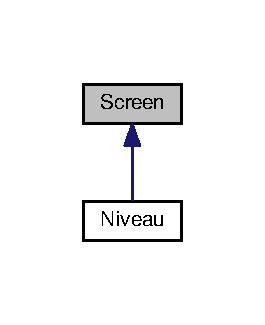
\includegraphics[width=127pt]{class_screen__inherit__graph}
\end{center}
\end{figure}
\subsection*{Public Member Functions}
\begin{DoxyCompactItemize}
\item 
virtual void \hyperlink{class_screen_a6933698ce05938524e1764fa42fe8129}{update} (float delta)=0
\begin{DoxyCompactList}\small\item\em Méthode appelée a chaque boucle de jeu. \end{DoxyCompactList}\item 
virtual void \hyperlink{class_screen_a7d3402d0cab593a375c84254b864ee22}{render} (float delta, S\+D\+L\+\_\+\+Renderer $\ast$rendu)=0
\begin{DoxyCompactList}\small\item\em Méthode appelée a chaque boucle de jeu. \end{DoxyCompactList}\end{DoxyCompactItemize}


\subsection{Detailed Description}
Classe representant un écran de jeu. 

Definition at line 18 of file Screen.\+hpp.



\subsection{Member Function Documentation}
\index{Screen@{Screen}!render@{render}}
\index{render@{render}!Screen@{Screen}}
\subsubsection[{\texorpdfstring{render(float delta, S\+D\+L\+\_\+\+Renderer $\ast$rendu)=0}{render(float delta, SDL_Renderer *rendu)=0}}]{\setlength{\rightskip}{0pt plus 5cm}virtual void Screen\+::render (
\begin{DoxyParamCaption}
\item[{float}]{delta, }
\item[{S\+D\+L\+\_\+\+Renderer $\ast$}]{rendu}
\end{DoxyParamCaption}
)\hspace{0.3cm}{\ttfamily [pure virtual]}}\hypertarget{class_screen_a7d3402d0cab593a375c84254b864ee22}{}\label{class_screen_a7d3402d0cab593a375c84254b864ee22}


Méthode appelée a chaque boucle de jeu. 


\begin{DoxyParams}{Parameters}
{\em delta} & \+: Temps écoulé depuis le dernier appel \\
\hline
{\em rendu} & \+: Pointeur vers le rendu courant \\
\hline
\end{DoxyParams}


Implemented in \hyperlink{class_niveau_acde898f3c32db22484bd9ee8a94ac124}{Niveau}.

\index{Screen@{Screen}!update@{update}}
\index{update@{update}!Screen@{Screen}}
\subsubsection[{\texorpdfstring{update(float delta)=0}{update(float delta)=0}}]{\setlength{\rightskip}{0pt plus 5cm}virtual void Screen\+::update (
\begin{DoxyParamCaption}
\item[{float}]{delta}
\end{DoxyParamCaption}
)\hspace{0.3cm}{\ttfamily [pure virtual]}}\hypertarget{class_screen_a6933698ce05938524e1764fa42fe8129}{}\label{class_screen_a6933698ce05938524e1764fa42fe8129}


Méthode appelée a chaque boucle de jeu. 


\begin{DoxyParams}{Parameters}
{\em delta} & \+: Temps écoulé depuis le dernier appel \\
\hline
\end{DoxyParams}


Implemented in \hyperlink{class_niveau_a287b7fc08a2d7102008c134a72462d4f}{Niveau}.



The documentation for this interface was generated from the following file\+:\begin{DoxyCompactItemize}
\item 
\hyperlink{_screen_8hpp}{Screen.\+hpp}\end{DoxyCompactItemize}

\hypertarget{class_space_intruders}{}\section{Space\+Intruders Class Reference}
\label{class_space_intruders}\index{Space\+Intruders@{Space\+Intruders}}


Classe representant le jeu.  




{\ttfamily \#include $<$Space\+Intruders.\+hpp$>$}

\subsection*{Public Member Functions}
\begin{DoxyCompactItemize}
\item 
\hyperlink{class_space_intruders_a7c53c28b660bb22a9433112768ded3ae}{Space\+Intruders} ()
\begin{DoxyCompactList}\small\item\em Construit la classe \hyperlink{class_space_intruders}{Space\+Intruders}. \end{DoxyCompactList}\item 
\hyperlink{class_space_intruders_a55184ccc75ec89b388b21d386f12fe07}{$\sim$\+Space\+Intruders} ()
\begin{DoxyCompactList}\small\item\em Detruit la classe \hyperlink{class_space_intruders}{Space\+Intruders}. \end{DoxyCompactList}\item 
int \hyperlink{class_space_intruders_a41016bf86ebd323141c427cb294fba44}{start} ()
\begin{DoxyCompactList}\small\item\em A utiliser pour lancer le jeu. \end{DoxyCompactList}\item 
void \hyperlink{class_space_intruders_afbdfd16308c83b984dba596c14c35203}{stop} ()
\begin{DoxyCompactList}\small\item\em A utiliser pour stopper le jeu. \end{DoxyCompactList}\item 
void \hyperlink{class_space_intruders_a6ed0614ff6dbdff01aff4d7512510148}{set\+Screen} (\hyperlink{class_screen}{Screen} $\ast$screen)
\begin{DoxyCompactList}\small\item\em Definit l\textquotesingle{}ecran courant du jeu. \end{DoxyCompactList}\item 
void \hyperlink{class_space_intruders_a8f305f7968abbb7fa54de664c4613902}{set\+Input\+Listener} (\hyperlink{class_input_listener}{Input\+Listener} $\ast$input)
\begin{DoxyCompactList}\small\item\em Definit la classe gérant les entrées. \end{DoxyCompactList}\item 
S\+D\+L\+\_\+\+Renderer $\ast$ \hyperlink{class_space_intruders_a506f579b9711c39716bdc7422835569c}{get\+Renderer} ()
\begin{DoxyCompactList}\small\item\em Accesseur du rendu. \end{DoxyCompactList}\item 
int \hyperlink{class_space_intruders_a1946136e897d33c5fadf06d4557d9d48}{getW} ()
\begin{DoxyCompactList}\small\item\em Accesseur de la largeur de la fenêtre. \end{DoxyCompactList}\item 
int \hyperlink{class_space_intruders_a76d5f27be1a2111de5355d84e9779036}{getH} ()
\begin{DoxyCompactList}\small\item\em Accesseur de la hauteur de la fenêtre. \end{DoxyCompactList}\end{DoxyCompactItemize}


\subsection{Detailed Description}
Classe representant le jeu. 

Definition at line 18 of file Space\+Intruders.\+hpp.



\subsection{Constructor \& Destructor Documentation}
\index{Space\+Intruders@{Space\+Intruders}!Space\+Intruders@{Space\+Intruders}}
\index{Space\+Intruders@{Space\+Intruders}!Space\+Intruders@{Space\+Intruders}}
\subsubsection[{\texorpdfstring{Space\+Intruders()}{SpaceIntruders()}}]{\setlength{\rightskip}{0pt plus 5cm}Space\+Intruders\+::\+Space\+Intruders (
\begin{DoxyParamCaption}
{}
\end{DoxyParamCaption}
)}\hypertarget{class_space_intruders_a7c53c28b660bb22a9433112768ded3ae}{}\label{class_space_intruders_a7c53c28b660bb22a9433112768ded3ae}


Construit la classe \hyperlink{class_space_intruders}{Space\+Intruders}. 



Definition at line 9 of file Space\+Intruders.\+cpp.

\index{Space\+Intruders@{Space\+Intruders}!````~Space\+Intruders@{$\sim$\+Space\+Intruders}}
\index{````~Space\+Intruders@{$\sim$\+Space\+Intruders}!Space\+Intruders@{Space\+Intruders}}
\subsubsection[{\texorpdfstring{$\sim$\+Space\+Intruders()}{~SpaceIntruders()}}]{\setlength{\rightskip}{0pt plus 5cm}Space\+Intruders\+::$\sim$\+Space\+Intruders (
\begin{DoxyParamCaption}
{}
\end{DoxyParamCaption}
)}\hypertarget{class_space_intruders_a55184ccc75ec89b388b21d386f12fe07}{}\label{class_space_intruders_a55184ccc75ec89b388b21d386f12fe07}


Detruit la classe \hyperlink{class_space_intruders}{Space\+Intruders}. 



Definition at line 12 of file Space\+Intruders.\+cpp.



\subsection{Member Function Documentation}
\index{Space\+Intruders@{Space\+Intruders}!getH@{getH}}
\index{getH@{getH}!Space\+Intruders@{Space\+Intruders}}
\subsubsection[{\texorpdfstring{get\+H()}{getH()}}]{\setlength{\rightskip}{0pt plus 5cm}int Space\+Intruders\+::getH (
\begin{DoxyParamCaption}
{}
\end{DoxyParamCaption}
)}\hypertarget{class_space_intruders_a76d5f27be1a2111de5355d84e9779036}{}\label{class_space_intruders_a76d5f27be1a2111de5355d84e9779036}


Accesseur de la hauteur de la fenêtre. 

\begin{DoxyReturn}{Returns}
Hauteur de la fenêtre 
\end{DoxyReturn}


Definition at line 115 of file Space\+Intruders.\+cpp.

\index{Space\+Intruders@{Space\+Intruders}!get\+Renderer@{get\+Renderer}}
\index{get\+Renderer@{get\+Renderer}!Space\+Intruders@{Space\+Intruders}}
\subsubsection[{\texorpdfstring{get\+Renderer()}{getRenderer()}}]{\setlength{\rightskip}{0pt plus 5cm}S\+D\+L\+\_\+\+Renderer $\ast$ Space\+Intruders\+::get\+Renderer (
\begin{DoxyParamCaption}
{}
\end{DoxyParamCaption}
)}\hypertarget{class_space_intruders_a506f579b9711c39716bdc7422835569c}{}\label{class_space_intruders_a506f579b9711c39716bdc7422835569c}


Accesseur du rendu. 

\begin{DoxyReturn}{Returns}
Renderer du jeu 
\end{DoxyReturn}


Definition at line 107 of file Space\+Intruders.\+cpp.

\index{Space\+Intruders@{Space\+Intruders}!getW@{getW}}
\index{getW@{getW}!Space\+Intruders@{Space\+Intruders}}
\subsubsection[{\texorpdfstring{get\+W()}{getW()}}]{\setlength{\rightskip}{0pt plus 5cm}int Space\+Intruders\+::getW (
\begin{DoxyParamCaption}
{}
\end{DoxyParamCaption}
)}\hypertarget{class_space_intruders_a1946136e897d33c5fadf06d4557d9d48}{}\label{class_space_intruders_a1946136e897d33c5fadf06d4557d9d48}


Accesseur de la largeur de la fenêtre. 

\begin{DoxyReturn}{Returns}
Largeur de la fenêtre 
\end{DoxyReturn}


Definition at line 111 of file Space\+Intruders.\+cpp.

\index{Space\+Intruders@{Space\+Intruders}!set\+Input\+Listener@{set\+Input\+Listener}}
\index{set\+Input\+Listener@{set\+Input\+Listener}!Space\+Intruders@{Space\+Intruders}}
\subsubsection[{\texorpdfstring{set\+Input\+Listener(\+Input\+Listener $\ast$input)}{setInputListener(InputListener *input)}}]{\setlength{\rightskip}{0pt plus 5cm}void Space\+Intruders\+::set\+Input\+Listener (
\begin{DoxyParamCaption}
\item[{{\bf Input\+Listener} $\ast$}]{input}
\end{DoxyParamCaption}
)}\hypertarget{class_space_intruders_a8f305f7968abbb7fa54de664c4613902}{}\label{class_space_intruders_a8f305f7968abbb7fa54de664c4613902}


Definit la classe gérant les entrées. 


\begin{DoxyParams}{Parameters}
{\em input} & \+: Classe gérant les entrées \\
\hline
\end{DoxyParams}


Definition at line 123 of file Space\+Intruders.\+cpp.

\index{Space\+Intruders@{Space\+Intruders}!set\+Screen@{set\+Screen}}
\index{set\+Screen@{set\+Screen}!Space\+Intruders@{Space\+Intruders}}
\subsubsection[{\texorpdfstring{set\+Screen(\+Screen $\ast$screen)}{setScreen(Screen *screen)}}]{\setlength{\rightskip}{0pt plus 5cm}void Space\+Intruders\+::set\+Screen (
\begin{DoxyParamCaption}
\item[{{\bf Screen} $\ast$}]{screen}
\end{DoxyParamCaption}
)}\hypertarget{class_space_intruders_a6ed0614ff6dbdff01aff4d7512510148}{}\label{class_space_intruders_a6ed0614ff6dbdff01aff4d7512510148}


Definit l\textquotesingle{}ecran courant du jeu. 


\begin{DoxyParams}{Parameters}
{\em screen} & \+: Ecran à afficher \\
\hline
\end{DoxyParams}


Definition at line 119 of file Space\+Intruders.\+cpp.

\index{Space\+Intruders@{Space\+Intruders}!start@{start}}
\index{start@{start}!Space\+Intruders@{Space\+Intruders}}
\subsubsection[{\texorpdfstring{start()}{start()}}]{\setlength{\rightskip}{0pt plus 5cm}int Space\+Intruders\+::start (
\begin{DoxyParamCaption}
{}
\end{DoxyParamCaption}
)}\hypertarget{class_space_intruders_a41016bf86ebd323141c427cb294fba44}{}\label{class_space_intruders_a41016bf86ebd323141c427cb294fba44}


A utiliser pour lancer le jeu. 



Definition at line 15 of file Space\+Intruders.\+cpp.

\index{Space\+Intruders@{Space\+Intruders}!stop@{stop}}
\index{stop@{stop}!Space\+Intruders@{Space\+Intruders}}
\subsubsection[{\texorpdfstring{stop()}{stop()}}]{\setlength{\rightskip}{0pt plus 5cm}void Space\+Intruders\+::stop (
\begin{DoxyParamCaption}
{}
\end{DoxyParamCaption}
)}\hypertarget{class_space_intruders_afbdfd16308c83b984dba596c14c35203}{}\label{class_space_intruders_afbdfd16308c83b984dba596c14c35203}


A utiliser pour stopper le jeu. 



Definition at line 103 of file Space\+Intruders.\+cpp.



The documentation for this class was generated from the following files\+:\begin{DoxyCompactItemize}
\item 
\hyperlink{_space_intruders_8hpp}{Space\+Intruders.\+hpp}\item 
\hyperlink{_space_intruders_8cpp}{Space\+Intruders.\+cpp}\end{DoxyCompactItemize}

\chapter{File Documentation}
\hypertarget{_input_listener_8hpp}{}\section{Input\+Listener.\+hpp File Reference}
\label{_input_listener_8hpp}\index{Input\+Listener.\+hpp@{Input\+Listener.\+hpp}}


Classe gérant les entrées.  


{\ttfamily \#include $<$S\+D\+L2/\+S\+D\+L.\+h$>$}\\*
{\ttfamily \#include $<$map$>$}\\*
Include dependency graph for Input\+Listener.\+hpp\+:
\nopagebreak
\begin{figure}[H]
\begin{center}
\leavevmode
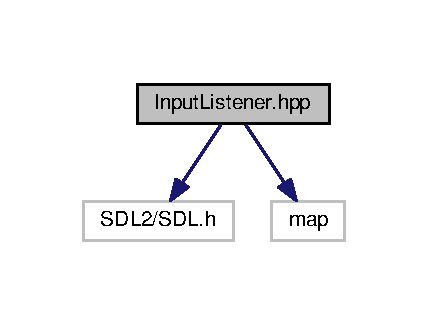
\includegraphics[width=206pt]{_input_listener_8hpp__incl}
\end{center}
\end{figure}
This graph shows which files directly or indirectly include this file\+:
\nopagebreak
\begin{figure}[H]
\begin{center}
\leavevmode
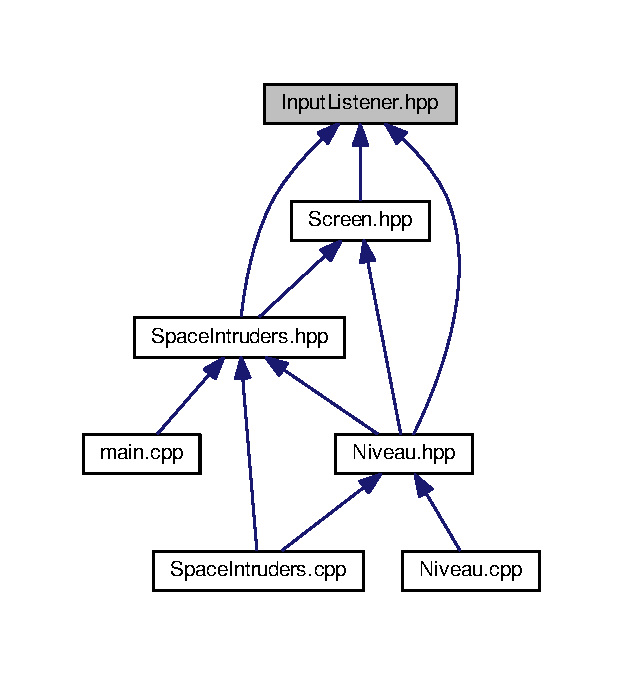
\includegraphics[width=299pt]{_input_listener_8hpp__dep__incl}
\end{center}
\end{figure}
\subsection*{Classes}
\begin{DoxyCompactItemize}
\item 
interface \hyperlink{class_input_listener}{Input\+Listener}
\begin{DoxyCompactList}\small\item\em Classe gérant les entrées. \end{DoxyCompactList}\end{DoxyCompactItemize}


\subsection{Detailed Description}
Classe gérant les entrées. 

\begin{DoxyAuthor}{Author}
Antoine Magnin, Pierre Caillaud 
\end{DoxyAuthor}
\begin{DoxyVersion}{Version}
0.\+1 
\end{DoxyVersion}

\hypertarget{main_8cpp}{}\section{main.\+cpp File Reference}
\label{main_8cpp}\index{main.\+cpp@{main.\+cpp}}
{\ttfamily \#include $<$S\+D\+L2/\+S\+D\+L.\+h$>$}\\*
{\ttfamily \#include $<$iostream$>$}\\*
{\ttfamily \#include \char`\"{}Space\+Intruders.\+hpp\char`\"{}}\\*
Include dependency graph for main.\+cpp\+:
\nopagebreak
\begin{figure}[H]
\begin{center}
\leavevmode
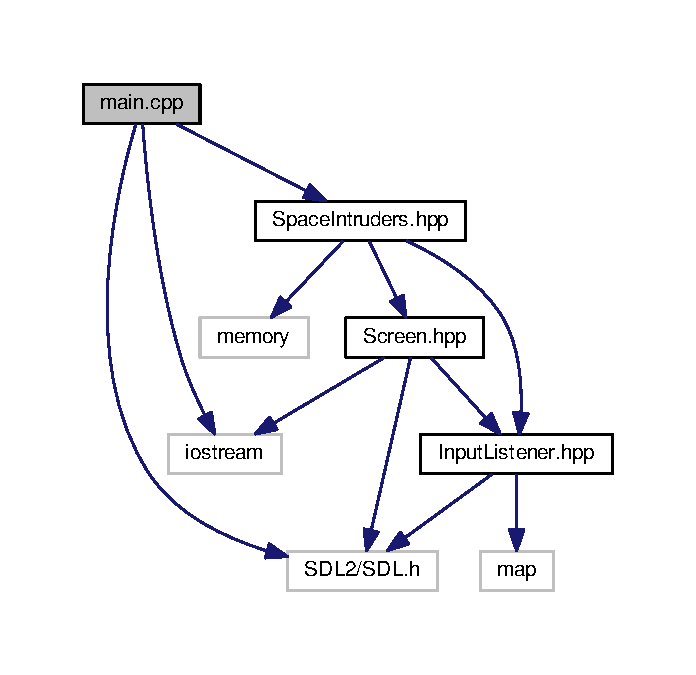
\includegraphics[width=334pt]{main_8cpp__incl}
\end{center}
\end{figure}
\subsection*{Functions}
\begin{DoxyCompactItemize}
\item 
int \hyperlink{main_8cpp_ae66f6b31b5ad750f1fe042a706a4e3d4}{main} ()
\end{DoxyCompactItemize}


\subsection{Function Documentation}
\index{main.\+cpp@{main.\+cpp}!main@{main}}
\index{main@{main}!main.\+cpp@{main.\+cpp}}
\subsubsection[{\texorpdfstring{main()}{main()}}]{\setlength{\rightskip}{0pt plus 5cm}int main (
\begin{DoxyParamCaption}
{}
\end{DoxyParamCaption}
)}\hypertarget{main_8cpp_ae66f6b31b5ad750f1fe042a706a4e3d4}{}\label{main_8cpp_ae66f6b31b5ad750f1fe042a706a4e3d4}


Definition at line 6 of file main.\+cpp.


\hypertarget{_niveau_8cpp}{}\section{Niveau.\+cpp File Reference}
\label{_niveau_8cpp}\index{Niveau.\+cpp@{Niveau.\+cpp}}
{\ttfamily \#include \char`\"{}Niveau.\+hpp\char`\"{}}\\*
{\ttfamily \#include $<$iostream$>$}\\*
Include dependency graph for Niveau.\+cpp\+:
\nopagebreak
\begin{figure}[H]
\begin{center}
\leavevmode
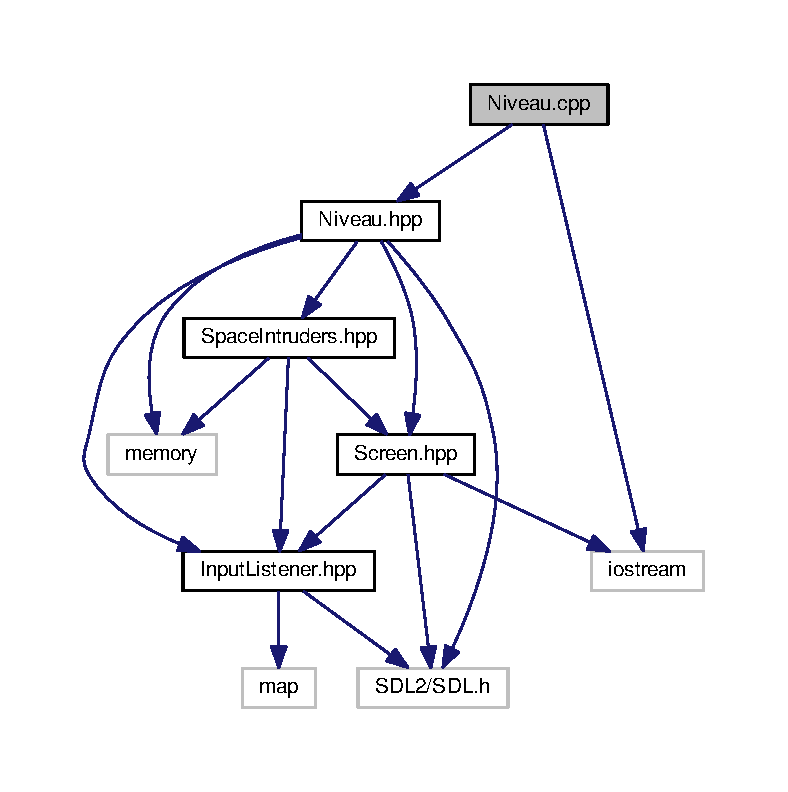
\includegraphics[width=350pt]{_niveau_8cpp__incl}
\end{center}
\end{figure}

\hypertarget{_niveau_8hpp}{}\section{Niveau.\+hpp File Reference}
\label{_niveau_8hpp}\index{Niveau.\+hpp@{Niveau.\+hpp}}


Classe représentant un niveau de jeu.  


{\ttfamily \#include $<$S\+D\+L2/\+S\+D\+L.\+h$>$}\\*
{\ttfamily \#include $<$memory$>$}\\*
{\ttfamily \#include \char`\"{}Screen.\+hpp\char`\"{}}\\*
{\ttfamily \#include \char`\"{}Input\+Listener.\+hpp\char`\"{}}\\*
{\ttfamily \#include \char`\"{}Space\+Intruders.\+hpp\char`\"{}}\\*
Include dependency graph for Niveau.\+hpp\+:
\nopagebreak
\begin{figure}[H]
\begin{center}
\leavevmode
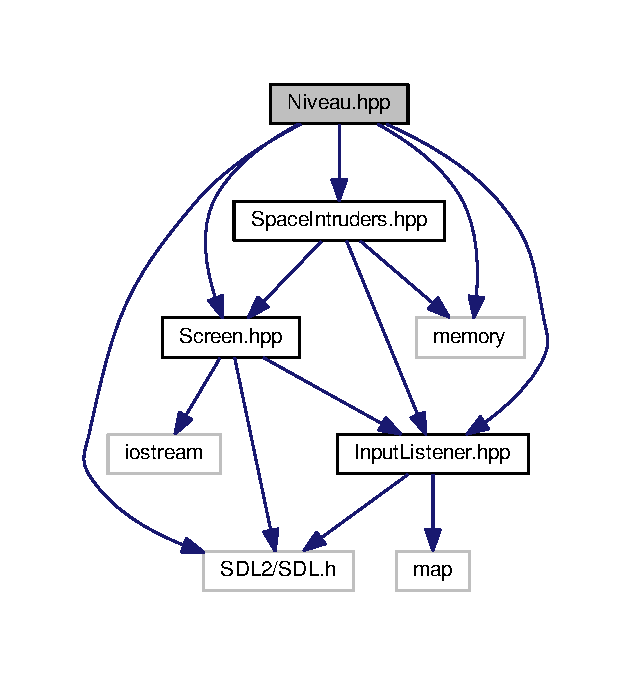
\includegraphics[width=303pt]{_niveau_8hpp__incl}
\end{center}
\end{figure}
This graph shows which files directly or indirectly include this file\+:
\nopagebreak
\begin{figure}[H]
\begin{center}
\leavevmode
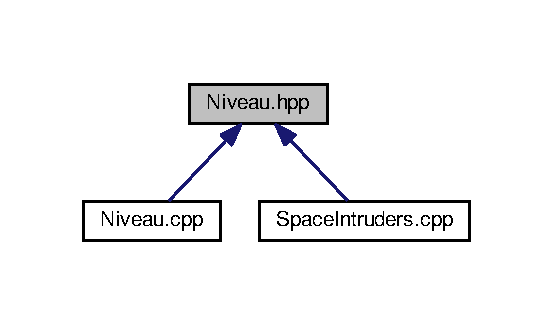
\includegraphics[width=266pt]{_niveau_8hpp__dep__incl}
\end{center}
\end{figure}
\subsection*{Classes}
\begin{DoxyCompactItemize}
\item 
class \hyperlink{class_niveau}{Niveau}
\begin{DoxyCompactList}\small\item\em Classe représentant un niveau de jeu. \end{DoxyCompactList}\end{DoxyCompactItemize}


\subsection{Detailed Description}
Classe représentant un niveau de jeu. 

\begin{DoxyAuthor}{Author}
Antoine Magnin, Pierre Caillaud 
\end{DoxyAuthor}
\begin{DoxyVersion}{Version}
0.\+1 
\end{DoxyVersion}

\hypertarget{_screen_8hpp}{}\section{Screen.\+hpp File Reference}
\label{_screen_8hpp}\index{Screen.\+hpp@{Screen.\+hpp}}


Classe représenatnt un écran de jeu.  


{\ttfamily \#include $<$S\+D\+L2/\+S\+D\+L.\+h$>$}\\*
{\ttfamily \#include $<$iostream$>$}\\*
{\ttfamily \#include \char`\"{}Input\+Listener.\+hpp\char`\"{}}\\*
Include dependency graph for Screen.\+hpp\+:
\nopagebreak
\begin{figure}[H]
\begin{center}
\leavevmode
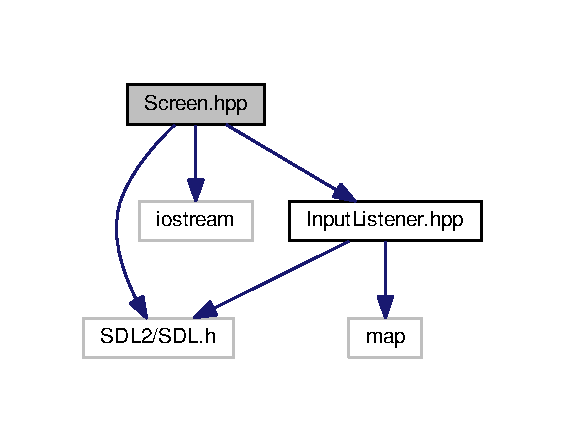
\includegraphics[width=271pt]{_screen_8hpp__incl}
\end{center}
\end{figure}
This graph shows which files directly or indirectly include this file\+:
\nopagebreak
\begin{figure}[H]
\begin{center}
\leavevmode
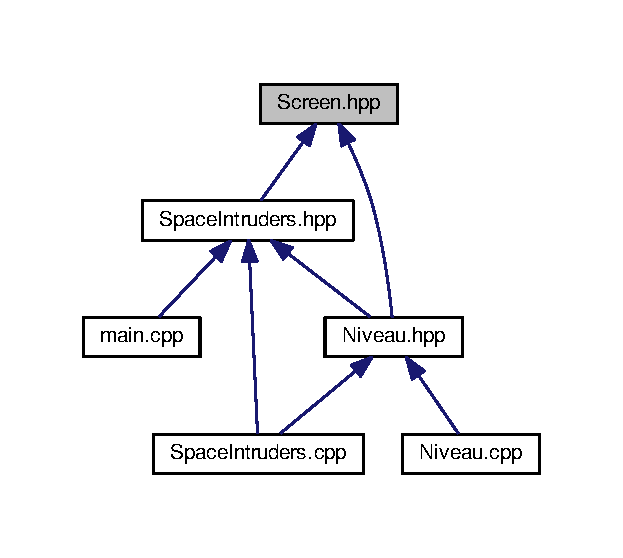
\includegraphics[width=299pt]{_screen_8hpp__dep__incl}
\end{center}
\end{figure}
\subsection*{Classes}
\begin{DoxyCompactItemize}
\item 
interface \hyperlink{class_screen}{Screen}
\begin{DoxyCompactList}\small\item\em Classe representant un écran de jeu. \end{DoxyCompactList}\end{DoxyCompactItemize}


\subsection{Detailed Description}
Classe représenatnt un écran de jeu. 

\begin{DoxyAuthor}{Author}
Antoine Magnin, Pierre Caillaud 
\end{DoxyAuthor}
\begin{DoxyVersion}{Version}
0.\+1 
\end{DoxyVersion}

\hypertarget{_space_intruders_8cpp}{}\section{Space\+Intruders.\+cpp File Reference}
\label{_space_intruders_8cpp}\index{Space\+Intruders.\+cpp@{Space\+Intruders.\+cpp}}
{\ttfamily \#include \char`\"{}Space\+Intruders.\+hpp\char`\"{}}\\*
{\ttfamily \#include $<$chrono$>$}\\*
{\ttfamily \#include $<$iostream$>$}\\*
{\ttfamily \#include $<$map$>$}\\*
{\ttfamily \#include \char`\"{}Niveau.\+hpp\char`\"{}}\\*
Include dependency graph for Space\+Intruders.\+cpp\+:
\nopagebreak
\begin{figure}[H]
\begin{center}
\leavevmode
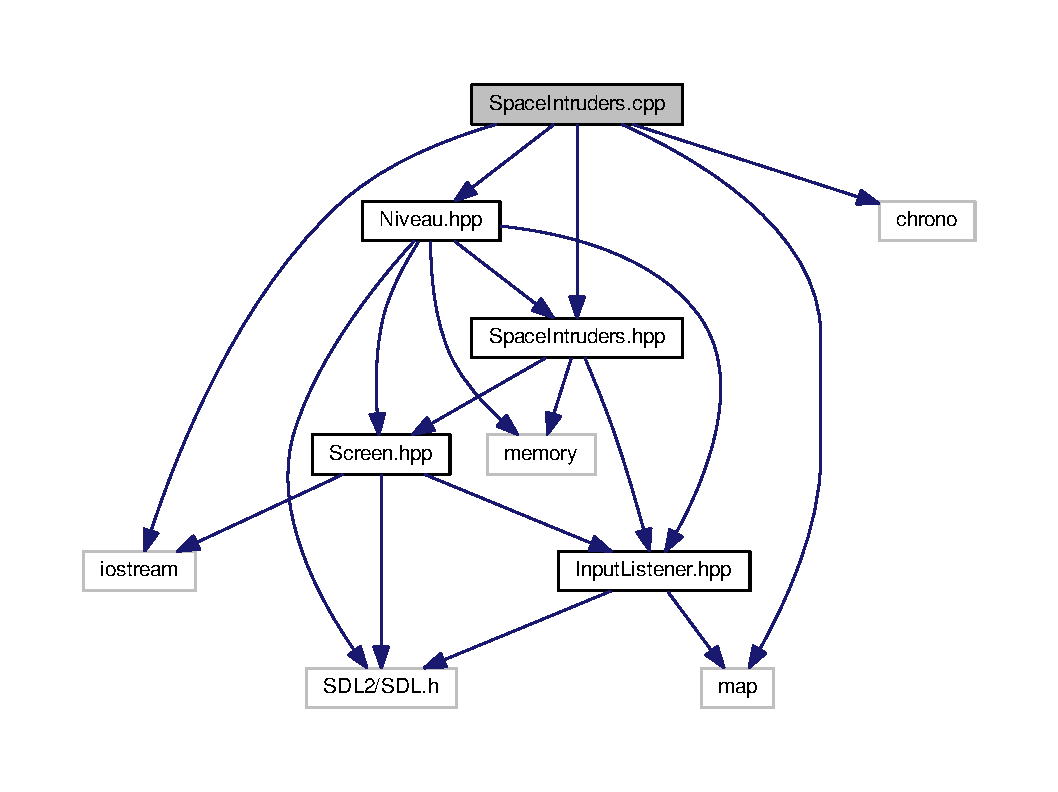
\includegraphics[width=350pt]{_space_intruders_8cpp__incl}
\end{center}
\end{figure}

\hypertarget{_space_intruders_8hpp}{}\section{Space\+Intruders.\+hpp File Reference}
\label{_space_intruders_8hpp}\index{Space\+Intruders.\+hpp@{Space\+Intruders.\+hpp}}


Classe principale du jeu.  


{\ttfamily \#include $<$memory$>$}\\*
{\ttfamily \#include \char`\"{}Screen.\+hpp\char`\"{}}\\*
{\ttfamily \#include \char`\"{}Input\+Listener.\+hpp\char`\"{}}\\*
Include dependency graph for Space\+Intruders.\+hpp\+:
\nopagebreak
\begin{figure}[H]
\begin{center}
\leavevmode
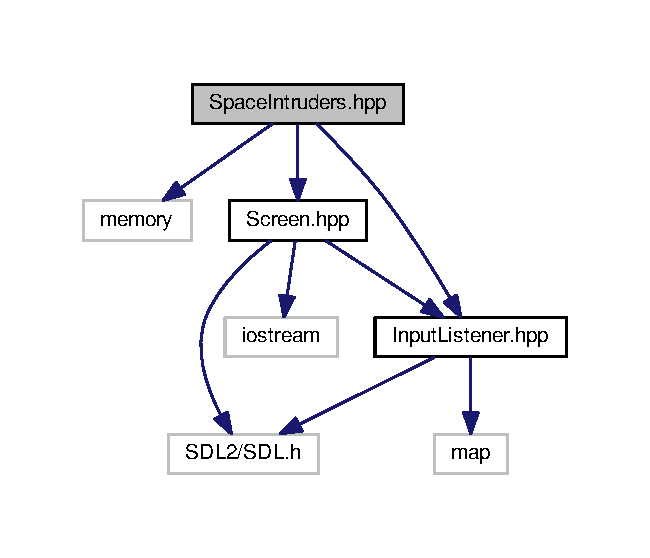
\includegraphics[width=312pt]{_space_intruders_8hpp__incl}
\end{center}
\end{figure}
This graph shows which files directly or indirectly include this file\+:
\nopagebreak
\begin{figure}[H]
\begin{center}
\leavevmode
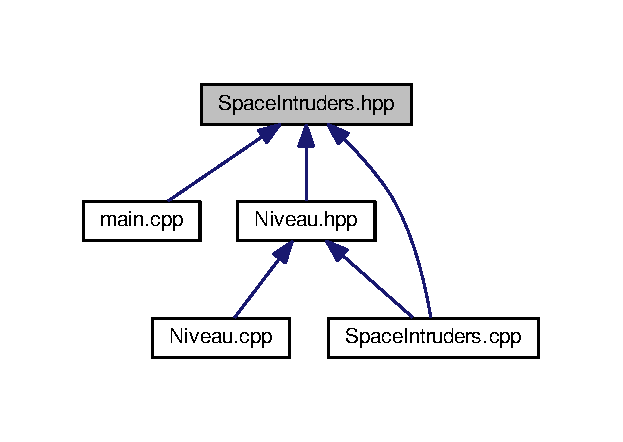
\includegraphics[width=299pt]{_space_intruders_8hpp__dep__incl}
\end{center}
\end{figure}
\subsection*{Classes}
\begin{DoxyCompactItemize}
\item 
class \hyperlink{class_space_intruders}{Space\+Intruders}
\begin{DoxyCompactList}\small\item\em Classe representant le jeu. \end{DoxyCompactList}\end{DoxyCompactItemize}


\subsection{Detailed Description}
Classe principale du jeu. 

\begin{DoxyAuthor}{Author}
Antoine Magnin, Pierre Caillaud 
\end{DoxyAuthor}
\begin{DoxyVersion}{Version}
0.\+1 
\end{DoxyVersion}

%--- End generated contents ---

% Index
\backmatter
\newpage
\phantomsection
\clearemptydoublepage
\addcontentsline{toc}{chapter}{Index}
\printindex

\end{document}
